

\def\>{\rangle}
\def\<{\langle}

\newcommand{\indicator}[1][A] {\mathbf{1}_{#1}} % Ensemble space


%TODO: decide whether the identity operator should be 1 or $I$ or something else

\chapter{Quantum mechanics}

% TODO: review classical uncertainty principle

\section{The postulates of quantum mechanics}

In this section we will review the standard formulations of quantum mechanics in terms of projective Hilbert spaces.

\subsubsection{Proposed nomenclature}

\begin{itemize}
	\item State vector $|\psi \> \in  \mathcal{H}$
	\item State $\psi \in  P(\mathcal{H})$
	\item Ensemble $\rho \in D(\mathcal{H})$
	
\end{itemize}

\subsubsection{Sketch of results}

Define BT as a set of ensembles that can be mixed.

The following are equivalent over BT
\begin{itemize}
	\item[QST-RAY] A pure quantum state is represented by a ray
	\item[QST-ENS] Ensembles are density operators (recover pure states as extreme points, recover ensembles as mixtures)
	\item[QST-SUBS] A pure state is a density operator with only one non-zero eigenvector (i.e. start with pure state representation directly in ensemble space)
	\item[QST-PROJ] A pure state is a projector
	\item[QST-EQ] A pure states is 
\end{itemize}

The following are equivalent over QST
\begin{itemize}
	\item[?] Superposition is multiple decomposition
	\item[?] The linearity of statistical mixing is a physical requirement. The linearity of the Hilbert space is a mathematical convenience.
	\item[?] The choice of a basis in the Hilbert space is a choice of a maximal set of orthogonal states plus a choice of gauge (i.e. a phase for each element of the basis).
\end{itemize}

The following are equivalent over QST
\begin{itemize}
	\item[BR-OBS] Expectations are defined for all observables and for all ensembles
	\item[BR-PROB] The probability of measuring a final state given an initial state is well-defined.
	\item[BR-ANG] The angles between pure states are well defined.
	\item[BR-ENT] The entropy is well-defined for all ensembles
\end{itemize}

Requires QST as base theory
\begin{itemize}
	\item 
\end{itemize}

The following are equivalent over QST+BR
\begin{itemize}
	\item[DR-SCEQ] The equation
	\item[DR-UNIT] Unitary evolution
	\item[DR-INN] Preservation of inner product
	\item[DR-NORM] Preservation of norm
	\item[DR-UBOR] Square of inner product infinitesimally close
	\item[DR-PERP] Perpendicular change
	\item[DR-OBAS] Preserves orthogonal basis
	\item[DR-EV] Deterministic and reversible evolution
	\item[DR-PROB] Probability distribution preserved
	\item[DR-INFO] The evolution preserves information entropy
\end{itemize}

Over QST+BR, PM $\implies$ DR-PSEQ and DR-MSEQ, and DR $\implies$ PM-DEQ
\begin{itemize}
	\item[DR-PSEQ] The evolution is quasi-static process
	\item[DR-MSEQ] The evolution is an infinite sequence of reversible measurements.
	\item[PM-DEQ] Projection measurements are process with equilibria that commute with a det/rev process.
\end{itemize}


\subsection{States}

The first postulate of quantum mechanics characterizes how states are represented in the mathematical framework.
\renewcommand{\thepostulate}{ST}
\begin{postulate}[State postulate]\label{rp_qm_postState}
	The state space of a quantum system is represented by the projective space $\mathrm{P}(\mathcal{H})$ of a complex Hilbert space $\mathcal{H}$. A state is represented by a ray of the Hilbert space $\mathcal{H}$. An ensemble is represented by a density operator $\rho : \mathcal{H} \to \mathcal{H}$, that is a positive semi-definite trace one self-adjoint operator.
\end{postulate}
\renewcommand{\thepostulate}{\Roman{assump}}
In terms of notation, we will mostly follow the convention most used by physicists,\footnote{Vectors will be noted as $|\psi\>$ instead by a simple letter $v$. The inner product will be noted as $\< \phi | \psi \> $, with a vertical line instead of a comma, and it will be linear in the first term instead of the second term. } with some addition or modification to make the connection to the math more clear. Mathematically, a complex Hilbert space $\mathcal{H}$ has three defining properties. It is a vector space, meaning that it is closed under addition $+ : \mathcal{H} \times \mathcal{H} \to \mathcal{H}$ and scalar multiplication $\cdot : \mathbb{C} \times \mathcal{H} \to \mathcal{H}$. It has an inner product, meaning that it is equipped with a map $\< \; \cdot \; | \; \cdot \; \> : \mathcal{H} \times \mathcal{H} \to \mathbb{C}$ that is positive-definite, linear in the second argument and conjugate symmetric. It is a complete metric space with respect to the distance function induced by the inner product, meaning that, given a sequence of vectors $|\psi_i\>$, if the series given by their norm $\sum_i |\psi_i|$ converges, then the series of given by the vectors $\sum_i |\psi_i\>$ converges as well. A ray of a Hilbert space is a one dimensional subspace. That is, given a vector $|\psi\>$, the corresponding ray is the set of all vectors given by $c |\psi\>$. With a slight abuse of notation, we will use $\psi$ to indicate the ray identified by the vector $|\psi\>$.

The second postulate of quantum mechanics characterizes observables.
\renewcommand{\thepostulate}{OBS}
\begin{postulate}[Observable postulate]\label{rp_qm_postObs}
	An observable is represented by a self-adjoint operator $O : \mathcal{H} \to \mathcal{H}$. Given a state $|\psi\>$, the expectation is given by $\<\psi | O | \psi \>$, and, given an ensemble $\rho$, the expectation is given by $\tr(O\rho)$.
\end{postulate}
\renewcommand{\thepostulate}{\Roman{assump}}

\renewcommand{\thepostulate}{PROJ}
\begin{postulate}[Projection measurement postulate]\label{rp_qm_postProjMeas}
	A projection measurement is defined by a set $M = \{\indicator[i]\}$ of projectors, representing the measurement outcomes, such that $\sum_i \indicator[i] = I$. If $|\psi\> \in \mathcal{H}$ represents the state before the measurement interaction, the ensemble after the interaction will be $\rho_{M} = \sum_i \indicator[i] \indicator[\psi]$ and the state after the measurement of the $i$-th outcome is $|\phi_i\> = \frac{\indicator[i]|\psi\>}{\sqrt{\< \psi | \indicator[i] | \psi \>}}$ with probability $\< \psi | \indicator[i] | \psi \>$. If $\rho$ is the ensemble before the measurement interaction, the ensemble after the interaction will be $\rho_{M} = \sum_i \indicator[i] \rho$ and the state after the measurement of the $i$-th outcome is $\hat{\rho}_i = \frac{\indicator[i] \rho}{\tr(\indicator[i] \rho)}$ with probability $\tr(\indicator[i] \rho)$.
\end{postulate}
\renewcommand{\thepostulate}{\Roman{assump}}

\renewcommand{\thepostulate}{UNIT}
\begin{postulate}[Time evolution postulate]\label{rp_qm_postUnitEvol}
	The time evolution of a state vector $|\psi\>$ is given by $d_t |\psi(t)\> = \frac{H}{\imath \hbar} |\psi(t)\>$ where $H$ is a self-adjoint operator. The time evolution of an ensemble $\rho$ is given by $d_t \rho = \left[\frac{H}{\imath\hbar}, \rho\right]$.
\end{postulate}
\renewcommand{\thepostulate}{\Roman{assump}}

\renewcommand{\thepostulate}{COMP}
\begin{postulate}[Composition postulate]\label{rp_qm_postComp}
	Given two quantum systems associated with the Hilbert spaces $\mathcal{H}_1$ and $\mathcal{H}_2$, their composite system is associates with the tensor product $\mathcal{H}_1 \otimes \mathcal{H}_2$.
\end{postulate}
\renewcommand{\thepostulate}{\Roman{assump}}



Review of the mathematical formulation of quantum mechanics
* wave-function (postulates - rays of Hilbert space)
- states are rays in Hilbert space
- observables are Hermitian operator inner product, Born rule, projection as final state
- composite systems (tensor product)
- unitary evolution
* mixtures and entropy

Composite system
* Show that system composition of quantum systems that is itself a quantum system gives the tensor product
* Review the arguments in the paper
* see if using a Segre embedding would make our life easier

\subsection{Bloch sphere review}

The state space of a two-state quantum system (i.e. qubit) is of fundamental importance as it allows us to visualize and therefore better understand almost all features of quantum mechanics. The space of pure states is isomorphic to a unit 2-sphere, with opposite points corresponding to orthogonal states, meaning that we can understand each pure state as a unit vector along a direction of three dimensional space. Since this is also the space of a spin 1/2 system, we will often label states as spatial directions. Let us quickly review the main features.

Let $|z^+\>$ and $|z^-\>$ be two orthonormal states, representing, for example, the two possible directions of spin along the vertical direction. Every other normalized state can be expressed as $\rho |z^+\> + \sqrt{1-\rho^2}e^{\imath \varphi} |z^-\>$ with $\rho \in [0,1]$ and $\varphi \in [0,2\pi)$. Normalization, in fact, imposes that the square of the norm of the coefficient sum to one. The arbitrariness of the phase allows us to impose the first coefficient to be real. Note that, for any $p \in (0,1)$, we can choose an arbitrary $\varphi$, meaning that we are choosing a point on a circle. At the endpoints $p \in \{0,1\}$, however, there is no longer a choice of $\varphi$. The topology, then, is the one of the sphere. We can therefore draw a sphere with $|z^+\>$ and $|z^-\>$ respectively at the top and at the bottom. The choice of $\rho$ will select a horizontal plane, whose intersection with the sphere will be a circle. The choice of $\varphi$ will pick a point on that circle. That is, $\rho$ and $\varphi$ can be understood as a sort of ``cylindrical coordinates over a sphere.'' We can also choose spherical coordinates $(\theta, \varphi)$ such that $\rho = \cos \theta$.

More remarkably, the interior points of the sphere represent mixed states. Therefore the whole space, the Bloch ball, represents the full space of ensembles for a two-state quantum systems. Given two ensembles $\rho_1$ and $\rho_2$, the statistical mixture $\rho = p \rho_1 + (1-p) \rho_2$ will be the point in between the two. The coefficient for each endpoint is higher the closer the mixture is to that point, meaning it is proportional to the distance to the other endpoint. That is,
\begin{equation}
	\rho = \frac{\overline{\rho \rho_2}}{\overline{\rho_1 \rho_2}} \rho_1 + \frac{\overline{\rho_1 \rho}}{\overline{\rho_1 \rho_2}} \rho_2.
\end{equation}

\section{States and ensembles}

As we have already seen in classical mechanics, re-expressing the same mathematical framework in different equivalent ways brings out new understanding. This will be even more clear in quantum mechanics, as the standard Hilbert space formulation is as good for calculations it is bad for understanding.

\subsection{Different Representations of pure states}
First of all, we should note that wave-functions do not provide a unique representation for states. The reader may already be aware that a change in norm or phase does not change the physics. Intuitively, all the physics is given by the born rule
\begin{equation}
	p(\phi|\psi) = \frac{\< \phi | \psi \>\< \psi | \phi \>}{\< \psi | \psi \>\< \phi | \phi \>}.
\end{equation}
If we chage $\psi$ with $\rho e^{\imath \theta} \psi$, we have
\begin{equation}
	p(\phi|\rho e^{\imath \theta}\psi) = \frac{\< \phi |\rho e^{\imath \theta}\psi \>\<\rho e^{\imath \theta}\psi | \phi \>}{\< \rho e^{\imath \theta}\psi | \rho e^{\imath \theta}\psi \>\< \phi | \phi \>} = \frac{\rho e^{\imath \theta}\rho e^{-\imath \theta}}{\rho e^{-\imath \theta}\rho e^{\imath \theta}}\frac{\< \phi | \psi \>\< \psi | \phi \>}{\< \psi | \psi \>\< \phi | \phi \>}=\frac{\< \phi | \psi \>\< \psi | \phi \>}{\< \psi | \psi \>\< \phi | \phi \>}.
\end{equation}

There is another detail, however, that is often neglected, maybe because it applies only to continuous variables. The inner production between two wave functions is given by:
\begin{equation}
	\< \phi | \psi \> = \int_X \phi^*(x) \psi(x) dx.
\end{equation}
Note that integrals do not change if we change the value of the wave-function over a set of measure zero. For example, if we changed $\psi(x)$ such had it returned zero over the rationals, the inner product wouldn't change. If the physics is given by the Born rule through the inner product, then the physics does not change. Mathematically, when we write the vector $|\psi \>$ we are actually talking about the set of all functions that are equivalent to the wave function $\psi(x)$. This is not something peculiar to quantum mechanics. In fact, this happens in classical probability as well. If we have a probability density $\rho(x,p)$, a change over a measure zero set will not change the expectation of any variable.

Since the representation in terms of Hilbert spaces already removes the second issue, is there a representation of states that eliminates the first as well? Turns out that there is. In a sense, working with Hilbert space is somewhat a conceptual no man's land. We are aware that we are dealing with probabilistic objects, but we are not really working with full fledged statistical mixtures. A lot things become clearer once we look at the quantum statistical framework as a whole and compare it to the classical statistical framework.

Let us look, then, at the space of all possible statistical mixtures. In quantum statistical mechanics, a state is represented by a density operator $\rho$. Mathematically, this is an operator $\rho : \mathcal{H} \to \mathcal{H}$ that is positive semi-definite trace one self-adjoint operator. In fact, since $\< \psi | \rho | \psi \>$ returns the probability to measure $\psi$ given the state $\rho$, $\rho$ is an observable. Since the probability cannot be negative, $\rho$ is positive semi-definite. Since the probability has to sum to one, it is a trace one operator.

Every pure state $\psi$ can be represented as the density operator $\rho_{\psi} = \frac{| \psi \> \< \psi |}{\< \psi | \psi \>}$. Note that, in fact, that $\rho_{\psi}$ is trace one and a change of phase will leave it unchanged. Also note that $\frac{| \psi \> \< \psi |}{\< \psi | \psi \>} = \indicator[\psi]$ is the projector corresponding by the subspace spanned by $\psi$.
\begin{insight}
	A state is equally represented by a ray $c|\psi\>$, by a density operator $\rho_{\psi}$ where $c|\psi\>$ is the only non-zero eigenvector, or by a the projector $\indicator[\psi]$ corresponding to the subspace $c|\psi\>$.
\end{insight}
We now have three equivalent ways to represent pure states.

\subsection{Two linearities: superposition and statistical mixing}

A linear combination, a superposition, $\sum c_i | \psi_i \>$ will give us another state, but is somewhat unclear what this operation means. First of all, we have the problem that the superposition is physically unique up to a total phase, so only the phase differences are physically significant. Moreover, the meaning of the norm of the coefficient $c_i$ is also ill defined. The overall intuition one gets is that $|c_i|^2$ corresponds to probability, but this does not actually work. In fact, we have
\begin{equation}
	\begin{aligned}
		|\phi\> &= c_1 |\psi_1\> + c_2 | \psi_2\> \\
		\< \phi | \phi\> &= |c_1|^2 \< \psi_1 |\psi_1\> + c_1^* c_2 \< \psi_1 |\psi_2\> + c_2^* c_1 \< \psi_2 |\psi_1\> + |c_2|^2 \< \psi_2 |\psi_2\> \\
		\< \psi_1 | \phi\> &= c_1 \< \psi_1 |\psi_1\> + c_2 \< \psi_1 |\psi_2\> \\
		p(\phi|\psi_1) &= \frac{\< \phi | \psi_1 \>\< \psi_1 | \phi \>}{\< \psi_1 | \psi_1 \>\< \phi | \phi \>} \\
		&= \frac{(c_1^* \< \psi_1 |\psi_1\> + c_2^* \< \psi_2 |\psi_1\>)(c_1 \< \psi_1 |\psi_1\> + c_2 \< \psi_1 |\psi_2\>)}{\< \psi_1 | \psi_1 \>(|c_1|^2 \< \psi_1 |\psi_1\> + c_1^* c_2 \< \psi_1 |\psi_2\> + c_2^* c_1 \< \psi_2 |\psi_1\> + |c_2|^2 \< \psi_2 |\psi_2\>)}.
	\end{aligned}
\end{equation}
In the special case where $\psi_1$ and $\psi_2$ are orthonormal, the above simplifies to
\begin{equation}
	p(\phi|\psi_1) = \frac{|c_1|^2}{|c_1|^2 + |c_2|^2}
\end{equation}
and therefore, if $|c_1|^2 + |c_2|^2 = 1$, we recover the probability. But this is a special case which does not work in general. And building our understanding on special cases that do not work in general is not a recipe for success.

We want to stress that superpositions play no fundamental role in classifying states: any state can be expressed as a linear combination of any other state. In a spin 1/2 system, for example, spin left is a linear combination of spin up and spin down with $|c_1|^2=|c_2|^2=\frac{1}{2}$. But spin up is also a linear combination of spin left and spin right with $|c_1|^2=|c_2|^2=\frac{1}{2}$. Any spin 1/2 state, in fact, can always be expressed as a linear combination of any two distinct states, not necessarily orthogonal. The reason is that any two linearly independent vectors of a two dimensional space will span the entire space.

We also want to stress that the linearity of superpositions is different from the linearity of statistical mixture. The first linearity acts on pure states only, uses complex coefficient, returns a pure state and is specific to quantum mechanics. The second linearity acts on all states, mixed or pure, uses real coefficient, returns mixed states and is present in both classical and quantum mechanics. In fact, it must be present in any physical theory, since all measurements are statistical in nature. If we pick two pure states $\psi$ and $\phi$ on the Bloch sphere for a spin 1/2 system, they will be represented by two points on the surface. The set of all superposition $c_{\psi}|\psi \> + c_{\phi} |\phi\>$ is the whole surface. The set of all statistical mixtures $p| \psi \> \< \psi | + (1-p) | \phi \> \< \phi |$, instead, is the line segment that contains the two points. Therefore, it is not true that superpositions are ``a kind of'' statistical mixture.

The two linearities, however, are related and understanding their relationship is key to understand why superpositions are possible in quantum mechanics but not in classical mechanics. Mathematically, if $|\phi\>$ is a superposition of $|\psi_1\>$ and $|\psi_2\>$, then we can find a statistical mixture $\rho$ of $|\psi_1\>\<\psi_1|$ and $|\psi_2\>\<\psi_2|$ such that it can also be expressed as a mixture of $|\phi\>\<\phi|$ and another state $|\hat{\phi}\>\<\hat{\phi}|$. Let $|\phi\> = c_1 |\psi_1\> + c_2 |\psi_2\>$. We define $|\hat{\phi}\> = c_1 |\psi_1\> - c_2 |\psi_2\>$. We have:
\begin{equation}
	\begin{aligned}
		| \phi \> \< \phi | &= c_1^* c_1 | \psi_1 \> \< \psi_1 | + c_1^* c_2 | \psi_1 \> \< \psi_2 | + c_2^* c_1 | \psi_2 \> \< \psi_1 | + c_2^* c_2 | \psi_2 \> \< \psi_2 | \\
		| \hat{\phi} \> \< \hat{\phi} | &= c_1^* c_1 | \psi_1 \> \< \psi_1 | - c_1^* c_2 | \psi_1 \> \< \psi_2 | - c_2^* c_1 | \psi_2 \> \< \psi_1 | + c_2^* c_2 | \psi_2 \> \< \psi_2 | \\
		| \phi \> \< \phi | &+ | \hat{\phi} \> \< \hat{\phi} | = 2 |c_1|^2 | \psi_1 \> \< \psi_1 | + 2 |c_2|^2 | \psi_2 \> \< \psi_2 |
	\end{aligned}
\end{equation}\begin{equation}
\begin{aligned}
	p_{\phi} &= \frac{\<\phi|\phi\>}{\<\phi|\phi\> + \<\hat{\phi}|\hat{\phi}\>} 
	&p_{\hat{\phi}} = \frac{\<\hat{\phi}|\hat{\phi}\>}{\<\phi|\phi\> + \<\hat{\phi}|\hat{\phi}\>} \\
	p_{1} &= \frac{2 |c_1|^2 \< \psi_1 | \psi_1 \> |}{\<\phi|\phi\> + \<\hat{\phi}|\hat{\phi}\>} 
	&p_{2} = \frac{2 |c_2|^2 \< \psi_2 | \psi_2 \> |}{\<\phi|\phi\> + \<\hat{\phi}|\hat{\phi}\>}
\end{aligned}
\end{equation}
\begin{equation}
	\begin{aligned}
		\rho = p_{\phi} \rho_{\phi} + p_{\hat{\phi}} \rho_{\hat{\phi}} &= \frac{\<\phi|\phi\>}{\<\phi|\phi\> + \<\hat{\phi}|\hat{\phi}\>} \frac{| \phi \> \< \phi |}{\< \phi | \phi \>} + \frac{\<\hat{\phi}|\hat{\phi}\>}{\<\phi|\phi\> + \<\hat{\phi}|\hat{\phi}\>} \frac{| \hat{\phi} \> \< \hat{\phi} |}{\< \hat{\phi} | \hat{\phi} \>} \\
		&=\frac{1}{\<\phi|\phi\> + \<\hat{\phi}|\hat{\phi}\>} \left(| \phi \> \< \phi | + | \hat{\phi} \> \< \hat{\phi} |\right) \\
		&=\frac{1}{\<\phi|\phi\> + \<\hat{\phi}|\hat{\phi}\>} \left(2 |c_1|^2 | \psi_1 \> \< \psi_1 | + 2 |c_2|^2 | \psi_2 \> \< \psi_2 |\right) \\
		&=\frac{2 |c_1|^2 \< \psi_1 | \psi_1 \> |}{\<\phi|\phi\> + \<\hat{\phi}|\hat{\phi}\>} \frac{| \psi_1 \> \< \psi_1 |}{\< \psi_1 | \psi_1 \>} + \frac{2 |c_2|^2 \< \psi_2 | \psi_2 \> |}{\<\phi|\phi\> + \<\hat{\phi}|\hat{\phi}\>} \frac{| \psi_2 \> \< \psi_2 |}{\< \psi_2 | \psi_2 \>} \\
		&=p_{1} \rho_{\psi_1} + p_{2} \rho_{\psi_2} \\
	\end{aligned}
\end{equation}
Note that $p_{\phi} + p_{\hat{\phi}}=1$, which means $\rho$ is a statistical mixture with the given probability. This also means that $p_1 + p_2 = 1$ as well. We therefore have a mixed state that can be expressed either as a mixture of $\psi_1$ and $\psi_2$ or of $\phi$ and $\hat{\phi}$.

The converse is also true. Suppose that $\rho = p_{\phi} \rho_{\phi} + p_{\hat{\phi}} \rho_{\hat{\phi}} = p_{1} \rho_{\psi_1} + p_{2} \rho_{\psi_2}$. Since $\rho$ is the mixture of two pure states, it is supported by a two dimensional subspace. Since $\rho$ is a mixture of $\rho_{\psi_1}$ and $\rho_{\psi_2}$, the subspace is the span of $\psi_1$ and $\psi_2$. Since $\phi$ must be in that subspace as well, it must be a superposition of $\psi_1$ and $\psi_2$. This means that $\phi$ is a superposition of $\psi_1$ and $\psi_2$ if and only if there is mixed state $\rho$ that can be expressed as a mixture of both $\psi_1$ and $\psi_2$ as well as a mixture of $\phi$ and some other state. This lead to the following:
\begin{insight}
	The existence of superpositions of pure states in quantum mechanics is equivalent to the existence of multiple decomposition of statistical mixtures in terms of pure states.
\end{insight}
This links the abstract operation of quantum superposition to the more concrete physical property of statistical mixing.

This explains why there are no superpositions in classical mechanics. Every classical ensemble has a unique decomposition in terms of pure states, where the pure states are limits of distributions all concentrated at a point in phase space. Since classical mechanics does not allow multiple decompositions, it does not allow superpositions either.

Note that the previous insight does not tell us that if a theory allows multiple decompositions then it must be equivalent to quantum mechanics. For example, if the state space of statistical mixture is a disc instead of a ball, we would still have multiple decompositions but no complex superpositions. It does tell us, however, that what superpositions are allowed is fixed by what mixtures are allowed, which means that the pure states are rays of a complex Hilbert space if and only if the space of statistical mixtures is isomorphic to the quantum one.

The above insight also tells us why quantum mechanics is a linear theory. If we have a physical process $\mathcal{P}$ that takes as input a statistical mixture, we expect that the output of the statistical mixture is the statistical mixture of the individual outputs. That is, $\mathcal{P}(p\rho_1 + (1-p) \rho_2) = p \mathcal{P}(\rho_1) + (1-p) \mathcal{P}(\rho_2)$. But if the process is linear with respect to statistical mixing, and the linearity of statistical mixing can be converted to the linearity of superpositions, then the process must be also linear with respect to superpositions. Similarly, if we have an observable $O$ and a statistical mixture, we expect that the expectation of the statistical mixture is the average of the expectations on the statistical components. That is $E[p\rho_1 + (1-p) \rho_2] = pE[\rho_1] + (1-p) E[\rho_2]$. In quantum mechanics, this means that $\tr(O(p\rho_1 + (1-p) \rho_2)) = p\tr(O\rho_1) + (1-p) \tr(O\rho_2)$. That is, the linearity of the observables is exactly the linearity of expectation values.

\subsection{The gap between the two linearities}

Note, however, that while the linearity of statistical mixture is a physically necessary requirement, the linearity of superposition is a choice dictated by mathematical convenience. As we saw, it is the Born rule that captures the physics, not the inner product. Therefore, a non-linear transformation that preserves the inner product is still physically valid. For example, consider the Bloch ball. Taken two orthogonal states $\psi$ and $\phi$, every other state can be expressed as a linear combination $c_{\psi} | \psi \> + c_{\phi} | \phi \>$. Now consider the map $m : \mathcal{H} \to \mathcal{H}$ defined by
\begin{equation}
	m(c_{\psi} | \psi \> + c_{\phi} | \phi \>) \mapsto e^{\imath \theta \frac{|c_{\phi}|}{\sqrt{|c_{\psi}|^2+|c_{\phi}|^2}}} ( c_{\psi} | \psi \> + c_{\phi}  | \phi \>),
\end{equation}
where $\theta \in (0,2\pi)$ is an arbitrary constant. The map is introducing a phase shift that is proportional to the cosine of the angle along the vertical direction. Since it is introducing only a total phase shift, it will map a vector to a physically equivalent vector. The physics will not change, and we do not expect the Born rule to change. However, since the shift is not linear, we will not expect the inner product to me conserved since only linear maps can preserve the inner product.

Let's verify all of this in the math. First, the map is colinear, meaning that it maps a ray to another ray. That is:
\begin{equation}
	\begin{aligned}
	m(k(c_{\psi} | \psi \> + c_{\phi} | \phi \>)) &= m(kc_{\psi} | \psi \> + k c_{\phi} | \phi \>) = e^{\imath \theta \frac{|kc_{\phi}|}{\sqrt{|kc_{\psi}|^2+|kc_{\phi}|^2}}} ( k c_{\psi} | \psi \> + k c_{\phi}  | \phi \>) \\
	&= k e^{\imath \theta \frac{|k||c_{\phi}|}{|k|\sqrt{|c_{\psi}|^2+|c_{\phi}|^2}}} ( c_{\psi} | \psi \> + c_{\phi}  | \phi \>) = k e^{\imath \theta \frac{|c_{\phi}|}{\sqrt{|c_{\psi}|^2+|c_{\phi}|^2}}} \left( c_{\psi} | \psi \> + c_{\phi}  | \phi \> \right) \\
	&= k \, m(c_{\psi} | \psi \> + c_{\phi} | \phi \>) \\
	\end{aligned}
\end{equation}
Moreover, we can see that each ray is mapped to the same ray. We can verify that the map in not linear. In fact:
\begin{equation}
	\begin{aligned}
		m(|\psi\>) &= |\psi\> \\
		m(|\phi\>) &=  e^{\imath \theta} | \phi \>\\
		m(|\psi\> + |\phi\>) &= e^{\frac{\imath \theta}{\sqrt{2}}}( |\psi\> +  | \phi \>) \neq |\psi\> + e^{\imath \theta} | \phi \>.
	\end{aligned}
\end{equation}
The inner product becomes:
\begin{equation}
	\begin{aligned}
	\<m(v) | m(w) \> &= e^{-\imath \theta \frac{|v_{\phi}|}{\sqrt{|v_{\psi}|^2+|v_{\phi}|^2}}} e^{\imath \theta \frac{|w_{\phi}|}{\sqrt{|w_{\psi}|^2+|w_{\phi}|^2}}} \< v | w \>,
	\end{aligned}
\end{equation}
which is manifestly not conserved. However, for the Born rule we have:
\begin{equation}
	\begin{aligned}
		\<m(v) | m(v) \> &= e^{-\imath \theta \frac{|v_{\phi}|}{\sqrt{|v_{\psi}|^2+|v_{\phi}|^2}}} e^{\imath \theta \frac{|v_{\phi}|}{\sqrt{|v{\psi}|^2+|v_{\phi}|^2}}} \< v | v \> = \< v | v \> \\
	p(m(v)|m(w)) &= \frac{\< m(v) | m(w) \>\< m(w) | m(v) \>}{\< m(v) | m(v) \>\< m(w) | m(w) \>} \\
	&= \frac{e^{-\imath \theta \frac{|v_{\phi}|}{\sqrt{|v_{\psi}|^2+|v_{\phi}|^2}}} e^{\imath \theta \frac{|w_{\phi}|}{\sqrt{|w_{\psi}|^2+|w_{\phi}|^2}}} \< v | w \> e^{-\imath \theta \frac{|w_{\phi}|}{\sqrt{|w_{\psi}|^2+|w_{\phi}|^2}}}e^{\imath \theta \frac{|v_{\phi}|}{\sqrt{|v_{\psi}|^2+|v_{\phi}|^2}}}  \< w | v \>}{\< v | v \>\< w | w \>} \\
		&= \frac{\< v | w \>\< w | v \>}{\< v | v \>\< w | w \>} = p(v|w).
	\end{aligned}
\end{equation}
As expected, the Born rule is conserved while the inner product is not.

This tells us that, technically, the linearity of the underlying vector space is not a physical requirement and, in principle, we could represent pure states with a space where superposition as ``slightly'' non-linear. That is, the fact that the space of pure states is a complex projective space is a physical requirement if we want to represent a set of states that provides the statistical mixtures given by quantum mechanics. However, using the underlying complex inner product space is not a physical requirement: it is mathematical convenience.

\begin{insight}
	The linearity of statistical mixing is a physical requirement. The linearity of the Hilbert space is a mathematical convenience.
\end{insight}

\subsection{Basis and gauge choice}

Once we decide to use the vector space, the representation of states in terms of vector is also defined up to an arbitrary choice. In a spin 1/2 system, for example, we typically define $|x^+\> = \frac{1}{\sqrt{2}} | z^+ \> + \frac{1}{\sqrt{2}} | z^- \>$. But note the state corresponding to spin down is the whole ray, so the above expression hides that fact that $|z^-\>$ hides a choice of arbitrary phase. We could, in fact, redefine $|z^-\>$ with a quarter of a turn phase shift, and have $|x^+\> = \frac{1}{\sqrt{2}} | z^+ \> + \imath \frac{1}{\sqrt{2}} | z^- \>$. In other words, the choice of representation of the physics in terms of the Hilbert space is up to an arbitrary choice of phase for elements of the basis.

For continuous observable, this choice is even more important, as it is not a matter of basis, but of operators. Suppose we have a wave function $\psi(x)$. The corresponding position and momentum operators will be $X=x$ and $P=-\imath \hbar \partial_x$. Now choose an arbitrary continuous function $\theta(x)$. This corresponds to an arbitrary choice of phase at each point. If we set $\phi(x) = e^{\imath \theta(x)} \psi(x)$, the probability distribution over position will not change as the norm at each point remains the same. If set $P_{\phi} = -\imath \hbar \partial_x - \hbar \partial_x \theta(x)$, we have
\begin{equation}
	\begin{aligned}
		\{X, P_{\phi}\} &= \{X, P - \hbar \partial_x \theta(x)\} = \{X, P \} - \{X, \hbar \partial_x \theta(x)\} = \{X, P \}
	\end{aligned}
\end{equation}
since $X$ will commute with any function of $x$. This means that $X$ and $P_{\theta}$ have the same commutation relationships than $X$ and $P$. Also note that
\begin{equation}
	\begin{aligned}
		\<\phi | P_{\phi} | \phi \> & = \int_X e^{ - \imath \theta} \psi(x) (-\imath \hbar \partial_x - \hbar \partial_x  \theta(x) )(e^{ \imath \theta} \psi(x)) dx \\
		& = \int_X e^{ - \imath \theta} \psi(x) (-\imath \hbar e^{ \imath \theta} \imath \partial_x \theta(x)  \psi(x) - e^{ \imath \theta} \imath \hbar \partial_x\psi(x)  - \hbar \partial_x  \theta(x) e^{ \imath \theta} \psi(x)) dx \\
		& = \int_X e^{ - \imath \theta} \psi(x) (- e^{ \imath \theta} \imath \hbar \partial_x\psi(x) ) dx \\
		& = \int_X \psi(x) (- \imath \hbar \partial_x )\psi(x)  dx  = \<\psi | P_{\psi} | \psi \>.
	\end{aligned}
\end{equation}
In other words, we can redefine both the phase of the wave function and the momentum operator so that the physics remains unchanged. This corresponds to the change of gauge we had in classical particle mechanics, where we could redefine momentum $p \to p + \partial f(x)$ while leaving the Poisson brackets, and therefore the space-time trajectories, unchanged.

\begin{insight}
	The choice of a basis in the Hilbert space is a choice of a maximal set of orthogonal states plus a choice of gauge (i.e. a phase for each element of the basis).
\end{insight}


To sum up, fixing the Hilbert space and its physical representation is equivalent to fixing the space of ensembles, including how they mix, requiring a linear representation in terms of the Hilbert space and choosing an arbitrary phase for each element of the spectrum of a complete set of observables.

\subsection{Probability from expectations}

Another interesting equivalence is the one between probability, subspaces and expectations. This equivalence exists also in classical probability, therefore we should understand it there fit. The standard way to define a probability space is by giving three objects. First, a sample space $\Omega$ that represents all the possible cases. In classical mechanics, it's phase space, where each point represent all the values of position and momentum. Second, an algebra of events $\Sigma_{\Omega}$ which represents all possible conditions we could test for. In classical mechanics, this is the collection of Borel sets, subsets of phase space that can be generated from the open regions using complements and countable unions. Third, a probability measure $p : \Sigma_{\Omega} \to [0,1]$ that associated a probability to each event. From this one can define random variables $X : \Omega \to \mathbb{R}$ and their expectation. That is, we start with a notion of probability and define a notion of observables on top.

We could proceed the other way. The key insight is that for every event $A \in \Sigma_{\Omega}$ we can define the indicator function $\indicator[A] : \Omega \to \{0,1\}$ that returns one if the given point is in $A$ or zero otherwise. This is a random variable and its expectation is exactly the probability of the event $A$. That is, $E[\indicator[A]] = p(A)$. Suppose, therefore, that we are given $\Omega$, $\Sigma_{\Omega}$ but not the probability measure. However, we are given the expectation operator $E : M(\Omega, \mathbb{R})$ that, given a function $f : \Omega \to \mathbb{R}$\footnote{The function will need to be measureable in the mathematical sense: the inverse image of a Borel set is a Borel set.}, $E[f]$ returns it's expectation. We can then define the probability measure as $p(A) = E[\indicator[A]]$.

A similar perspective can be achieved in quantum mechanics, and it is the basis of some other axiomatic approaches and quantum reconstruction approaches, like quantum logic. As we are using the same notation for indicator functions and projectors, it should not be surprising that projectors play the role of indicator function in quantum mechanics. A projector $P$ is an idempotent linear operator, meaning that $P^2 = P$. This also means that $E[P^2] = E[P]$. This is true for an indicator function $I$ as well: since the only values $I$ takes are zeros and one, $I^2=I$, and $E[I^2] = E[I]$. On the other hand, the spectrum of a projector (i.e. the possible eigenvalues) consists only of zero and one, just like an indicator function. Therefore, if we can reverse the definitions for probability in quantum mechanics as well.

The standard construction starts with a set of pure states $\mathbf{P}(\mathcal{H})$, defines the Born rule $p(\phi | \psi)$ in terms of the inner product, and then the expectation based on the Born rule. We can start with a set of pure states $\mathbf{P}(\mathcal{H})$, where $\mathcal{H}$ is taken as a vector space forgetting its inner product, the space of all possible observables $O(\mathcal{H})$ and the expectation operator $E : O(\mathcal{H}) \to \mathbb{R}$. For every pure state $\phi \in \mathbf{P}(\mathcal{H})$ we can find the corresponding projector $\indicator[\phi]$ and define $p(\phi) = E[\indicator[\phi]]$. This allows to reconstruct the mixed state, much like we reconstructed the probability measure in classical mechanics. To reconstruct the Born rule, for each pure $\psi \in \mathbf{P}(\mathcal{H})$ we need an $E_{\psi}$ that gives us the expectations of all the variables if we prepared $\psi$. Then we can set $p(\phi | \psi) = E_{\psi}[\indicator[\phi]]$.

Therefore condition
\begin{equation}\label{rp-qm-br-condExpectations}
	\tag{BR-EXP}
	\eqtext{Expectations are defined for all observables and for all ensembles} 
\end{equation}
is an alternative characterization of the Born rule.

\subsection{Born rule and angles in projective space}

As we saw, the Born rule is essentially a relationship between rays, points in the projective space. We want to understand what exactly is it describing. Since it is a relationship between two pure states, let us take two rays $\psi, \phi \in P(\mathcal{H})$. Regardless of the dimensionality of $\mathcal{H}$, $\psi$ and $\phi$ will span a two-dimensional subspace, a Bloch sphere. In fact, considering the circle that contains $\psi$, $\phi$ and its opposite  $\phi_{\perp}$ will suffice.

Since $\phi$ and $\phi_{\perp}$ are opposite in the Bloch sphere, and therefore orthogonal, we can write $|\psi\> = \rho |\phi\> + \sqrt{1-\rho^2}e^{\imath \theta} |\phi_{\perp}\>$. We have
\begin{equation}
	\begin{aligned}
		p(\psi|\phi) &= \frac{\< \phi | \psi \>\< \psi | \phi \>}{\< \psi | \psi \>\< \phi | \phi \>} = \rho^2 = \cos^2 \theta_{\psi\phi} \\
		\theta_{\psi\phi} &= \arccos \sqrt{\frac{\< \phi | \psi \>\< \psi | \phi \>}{\< \psi | \psi \>\< \phi | \phi \>}}.
	\end{aligned}
\end{equation}
In other words, the Born rule defines the geometry of the projective space by defining the angles between points. Note that, since we are on a unit sphere, the angle can be understood also as a distance along the maximal circle that connects the two. The maximal circles are the geodesics of the sphere and therefore the angle is the distance between the points. Therefore $\theta_{\psi\phi}$ is literally the distance function that define the geometry of the space.\footnote{The angle is the distance as calculated using the \href{https://en.wikipedia.org/wiki/Fubini\%E2\%80\%93Study_metric\#In_bra-ket_coordinate_notation}{Fubini-Study metric}.} We have that
\begin{equation}\label{rp-qm-br-condAngles}
	\tag{BR-ANG}
	\eqtext{The angles between pure states are well defined.} 
\end{equation}
is an alternative characterization of the Born rule.


\subsection{Entropy and the Born rule}

TODO: preamble. 


\begin{figure}[H]
	\centering
	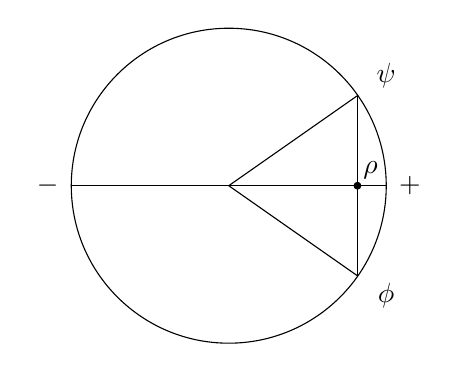
\begin{tikzpicture}[scale = 1]
		\draw (0,0) circle (2);
		\node at (-2.3,0) {$-$};
		\node at (2.3,0) {$+$};
		\node at (2,1.4) {$\psi$};
		\node at (2,-1.4) {$\phi$};
		\draw (-2,0) -- (2,0);
		\begin{scope}
			\clip(0,0) circle (2);
			\draw (0,0) -- (2,1.4);
			\draw (0,0) -- (2,-1.4);
			\draw (1.634,1.4) -- (1.634,-1.4);
		\end{scope}
		\fill (1.634,0) circle (0.05);
		\node at (1.8,.2) {$\rho$};
	\end{tikzpicture}
	\caption{Geometric diagonalization of an equal mixture of two states.}\label{rp-qm-geometricDiagonalization}
\end{figure}

To calculate the entropy of a mixture of two pure states, we can use the understanding that we built in terms of ensembles and their multiple decomposition. Let $\psi$ and $\phi$ be two pure states. Their equal mixture $\rho=\frac{1}{2}\rho_{\psi} + \frac{1}{2}\rho_{\phi}$ will be the midpoint between them. To calculate the entropy, we need to diagonalize $\rho$ and calculate the Shannon entropy from the eigenvalues. To diagonalize $\rho$ we need to express it as a mixture of two orthogonal $+$ and $-$. But $+$ and $-$ will be orthogonal only if they are opposite points on the Bloch sphere. Therefore, $\rho$ is diagonalized by $+$ and $-$ if and only if it lies on the axis identified by $+$ and $-$ as we see in figure \ref{rp-qm-geometricDiagonalization}. Geometrical, we will have $\rho = \frac{\overline{-\rho}}{\overline{-+}}\rho_{+} + \frac{\overline{\rho+}}{\overline{-+}}\rho_{-}$. Using simple trigonometry and recalling the relationship between the Born rule and angles, we have:
\begin{equation}
	\begin{aligned}
		\cos \theta_{\psi+} &= \cos \frac{\theta_{\psi\phi}}{2} = \sqrt{p(\phi|\psi)} \\
		\rho &= \frac{\overline{-\rho}}{\overline{-+}}\rho_{+} + \frac{\overline{\rho+}}{\overline{-+}}\rho_{-} = \frac{1+\cos \theta_{\psi+}}{2}\rho_{+} + \frac{1-\cos \theta_{\psi+}}{2}\rho_{-} \\
		&= \frac{1+\sqrt{p(\phi|\psi)}}{2}\rho_{+} + \frac{1-\sqrt{p(\phi|\psi)}}{2}\rho_{-}.
	\end{aligned}
\end{equation}


\begin{figure}
	\centering
	\begin{tikzpicture}
		\def\xi{0.25};
		\def\vi{1.25};
		\def\m{1};
		\def\b{1};
		\pgfplotsset{ticks=none}
		\begin{axis}[
			width=5.3cm,
			height=4.5cm,				
			axis lines=middle,
			axis line style={-},
			clip=false,
			xlabel=$p(\phi | \psi)$,
			xlabel style={below=5pt},
			ylabel=$S\left(\frac{1}{2} \rho_{\phi} + \frac{1}{2} \rho_{\psi}\right)$,
			ylabel style={above=2pt, left},
			xmin=0,xmax=1.1,
			ymin=0,ymax=0.8,
			domain=0:4,
			]
			\addplot[black,samples=69]{ - ((1+sqrt(x))/2) * ln((1+sqrt(x))/2) - ((1-sqrt(x))/2) * ln((1-sqrt(x))/2)}
			node [pos=0,left] {$1$};
		\end{axis}
	\end{tikzpicture}
	\caption {Entropy of a mixture of two pure states as a function of their Born rule.} \label{fig_rp_qm_entropyVsProb}
\end{figure}


The entropy is therefore
\begin{equation}
	\begin{aligned}
		S(\rho) = - \tr(\rho \log \rho) = - \frac{1+\sqrt{p(\phi|\psi)}}{2} \log \frac{1+\sqrt{p(\phi|\psi)}}{2} - \frac{1-\sqrt{p(\phi|\psi)}}{2} \log \frac{1-\sqrt{p(\phi|\psi)}}{2}.
	\end{aligned}
\end{equation}
The relationship is plotted in figure \ref{fig_rp_qm_entropyVsProb} and, as one can see, it is strictly concave. The relationship is, therefore, invertible: if we are given the entropy of all pairs of state we would be able to recover the Born rule. In other words
\begin{equation}\label{rp-qm-br-condEntropy}
	\tag{BR-ENT}
	\eqtext{The entropy is well defined for all ensembles} 
\end{equation}
is an alternative characterization of the Born rule.


States are rays <-> states are pure ensembles.

Probability as expectations of indicator functions

Projections as indicator functions

Orthogonality as mutual exclusivity

Inner product as overlap between pure ensembles

\section{Schroedinger equation and unitary evolution}

We start with the Schroedinger equation
\begin{equation}\label{rp-qm-uev-condSchroedingerEq}
	\tag{DR-SCEQ}
	\eqtext{The evolution follows the equation $\imath \hbar \frac{d}{dt} \psi(t) = H \psi(t)$ where $H$ is a self-adjoint operator}
\end{equation}

\subsection{Infinitesimal time evolution}

The Schroedinger equation describes time evolution as a relationship between the change of the state and the Hamiltonian of the system. Here we want to characterize time evolution as a map $U_{dt}$ that takes the state at time $t$ and returns the state at time $t + dt$. We have
\begin{equation}
	\begin{aligned}
		\psi(t+dt) &= \psi(t) + d\psi(t) = \psi(t) + \frac{d}{dt} \psi(t) dt = \psi(t)+ \frac{H dt}{\imath \hbar} \psi(t)\\
		&= \left(1 + \frac{H dt}{\imath \hbar}\right)\psi(t) = U_{dt}\psi(t).
	\end{aligned}
\end{equation}
Since $H$ is a self-adjoint operator, we have
\begin{equation}
	\begin{aligned}
		U_{dt}^\dagger U_{dt} &= \left(1 + \frac{H dt}{\imath \hbar}\right)^\dagger \left(1 + \frac{H dt}{\imath \hbar}\right) = \left(1 + \frac{H^\dagger dt}{(- \imath) \hbar}\right) \left(1 + \frac{H dt}{\imath \hbar}\right) = \left(1 - \frac{H dt}{\imath \hbar}\right) \left(1 + \frac{H dt}{\imath \hbar}\right) \\
		&= 1 + \left(\frac{H dt}{\imath \hbar}\right)^2 = 1 + O(dt^2).
	\end{aligned}
\end{equation}
This means that the infinitesimal time evolution operator $U_{dt}$ is unitary.

We can proceed in the opposite way. Given an infinitesimal unitary time evolution operator, we can recover the change of the state in time.
\begin{equation}
	\begin{aligned}
		\frac{d\psi(t)}{dt} &= \frac{\psi(t+dt) - \psi(t)}{dt} = \frac{U_{dt}\psi(t) - \psi(t)}{dt} = \frac{U_{dt} - 1}{dt} \psi(t) = A \psi(t)\\
		U_{dt} &= 1 + A dt
	\end{aligned}
\end{equation}
From the unitarity we have
\begin{equation}
	\begin{aligned}
		U_{dt}^\dagger U_{dt} &= \left(1 + A dt\right)^\dagger \left(1 + A dt\right) = \left(1 + A^\dagger dt\right) \left(1 + A dt\right) = 1 + \left(A + A^\dagger\right)dt + A^\dagger A dt^2 \\
		&= 1 + \left(A + A^\dagger\right)dt + O(dt^2) = 1 \\
		A &= - A^\dagger
	\end{aligned}
\end{equation}
Therefore $A$ is skew-adjoint, and we can set $A = \frac{H}{\imath \hbar}$ where $H$ is a self-adjoint operator. Therefore $\imath \hbar \frac{d}{dt} \psi(t) = \imath \hbar A \psi(t) = H \psi(t)$. The evolution follows the Schroedinger equation. To sum it up
\begin{equation}\label{rp-qm-uev-condUnitaryEvolution}
	\tag{DR-UNIT}
	\eqtext{Time evolution is unitary: $U^{\dagger}_{dt} U_{dt} = U_{dt} U^{\dagger}_{dt} = 1$} 
\end{equation}
is equivalent to \ref{rp-qm-uev-condSchroedingerEq}.

TODO: make sure to discuss the invertibility condition!

Note that if the evolution is unitary, then the inner product is conserved. In fact
\begin{equation}
	\begin{aligned}
		\< U_{dt} \phi | U_{dt} \psi\> &= \< \phi | U^\dagger_{dt} U_{dt} | \psi \> =\<  \phi | \psi \>.
	\end{aligned}
\end{equation}
The argument works in reverse as well: an infinitesimal time evolution operator that conserves the inner product is unitary. Therefore
\begin{equation}\label{rp-qm-uev-condInnerProductPreserved}
	\tag{DR-INN}
	\eqtext{Time evolution preserves the inner product : $\< U_{dt} \phi | U_{dt} \psi\> =\<  \phi | \psi \>$} 
\end{equation}
is equivalent to \ref{rp-qm-uev-condUnitaryEvolution}.

In particular, unitary evolution will preserve the norm of vectors, since $|\psi|^2 = \<\psi | \psi \>$. Note that the inner product can be expressed, through the polarization identity, in terms of the norm.
\begin{equation}
	\begin{aligned}
		\< \phi | \psi \> = \frac{1}{4}\left( |\phi + \psi|^2 - |\phi - \psi|^2 - \imath |\phi + \imath \psi|^2 +\imath |\phi - \imath \psi|^2 \right)
	\end{aligned}
\end{equation}
If $U_{dt}$ is a linear transformation that preserves the norm, that is $|U_{dt} \psi | ^2 = | \psi |^2$, then, we have
\begin{equation}
	\begin{aligned}
		\< U_{dt} \phi | U_{dt} \psi \> &= \frac{1}{4}\left( |U_{dt}\phi + U_{dt}\psi|^2 - |U_{dt}\phi - U_{dt}\psi|^2 - \imath |U_{dt}\phi + \imath U_{dt}\psi|^2 +\imath |U_{dt}\phi - \imath U_{dt}\psi|^2 \right) \\
		&= \frac{1}{4}\left( |U_{dt}(\phi + \psi)|^2 - |U_{dt}(\phi - \psi)|^2 - \imath |U_{dt}(\phi + \imath \psi)|^2 +\imath |U_{dt}(\phi - \imath \psi)|^2 \right) \\
		&= \frac{1}{4}\left( |\phi + \psi|^2 - |\phi - \psi|^2 - \imath |\phi + \imath \psi|^2 +\imath |\phi - \imath \psi|^2 \right) =  \< \phi | \psi \> 
	\end{aligned}
\end{equation}
Therefore condition
\begin{equation}\label{rp-qm-uev-condNormalized}
	\tag{DR-NORM}
	\eqtext{Time evolution is linear and preserves the norm: $\< \psi(t) | \psi(t) \> = \< \psi(t+dt) | \psi(t+dt) \>$} 
\end{equation}
is equivalent to condition \ref{rp-qm-uev-condInnerProductPreserved}.

We now look at the square of the inner product between two states infinitesimally close in time. We have
\begin{equation}
	\begin{aligned}
		|\<\psi(t) | \psi(t + dt)\>|^2 &= \< \psi(t) | U_{d t} \psi(t)\> \< U_{d t} \psi(t) | \psi(t)\> \\
		&=\<  \psi(t) | 1 + \frac{H dt}{\imath \hbar} | \psi(t)\> \<\psi(t) | \left(1 + \frac{H dt}{\imath \hbar} \right)^{\dagger}| \psi(t)\> \\
		&=\<  \psi(t) | 1 + \frac{H dt}{\imath \hbar} | \psi(t)\> \<\psi(t) | 1 - \frac{H dt}{\imath \hbar} | \psi(t)\> \\
		&=\< \psi(t) | \psi(t)\> \< \psi(t) | \psi(t)\> + \<  \psi(t) | \psi(t)\> \<\psi(t) | - \frac{H dt}{\imath \hbar} | \psi(t)\> \\
		&+ \< \psi(t) | \frac{H dt}{\imath \hbar} | \psi(t)\> \<\psi(t) | \psi(t)\> + O(dt^2)\\
		&=|\<\psi(t) | \psi(t)\>|^2 + O(dt^2).
	\end{aligned}
\end{equation}
In particular, if the vector is normalized, we have
\begin{equation}
	\begin{aligned}
		|\<\psi(t) | \psi(t + dt)\>|^2 &= 1 + O(dt^2).
	\end{aligned}
\end{equation}
That is, the square of the inner product between two infinitesimally close states is one.

For the converse, let's assume $U_{dt}$ is such that $|\<\psi(t) | \psi(t + dt)\>|^2 = |\<\psi(t) | \psi(t)\>|^2$. As we saw before, since $U_{dt}$ is infinitesimal, we can write $U_{dt} = 1 + A dt$. We have:
\begin{equation}
	\begin{aligned}
		|\<\psi(t) | \psi(t)\>|^2 &= |\<\psi(t) | \psi(t + dt)\>|^2 = \<  \psi(t) | U_{dt} \psi(t)\> \< U_{dt} \psi(t) | \psi(t)\> \\
		&= \<  \psi(t) | U_{dt} | \psi(t)\> \<  \psi(t) | U_{dt}^{\dagger} | \psi(t)\> \\
		&= \<  \psi(t) | 1 + A dt | \psi(t)\> \<  \psi(t) | 1 + A^{\dagger} dt | \psi(t)\> \\
		&=|\<\psi(t) | \psi(t)\>|^2 + \<\psi(t) | \psi(t)\> \<  \psi(t) | (A + A^{\dagger}) dt | \psi(t)\> + O(dt^2).
	\end{aligned}
\end{equation}
This means that $A = A^{\dagger}$ and therefore $U_{dt} = 1 + A dt$ is unitary. Therefore condition
\begin{equation}\label{rp-qm-uev-condUnitaryBorn}
	\tag{DR-UBOR}
	\eqtext{The square of the inner product between to states infinitesimally close in time is one: $|\< \psi(t) | \psi(t + dt) \> |^2 = 1$} 
\end{equation}
is yet another equivalent condition to unitary evolution.

The above two conditions make sense if we understand what happens geometrically. A unitary evolution is effectively a rotation in the Hilbert space, that is why the norm is conserved. An infinitesimal unitary evolution, then, is an infinitesimal rotation so the change is tangent to the circle, and therefore perpendicular with respect to the original vector. This is why the projection of the new vector onto the old one is equal to the norm.

However, perpendicular does not mean orthogonal in this case. In the complex plane, a multiplication by $\imath$ gives us a perpendicular vector that is not orthogonal with respect to the inner product. To see this
\begin{equation}
	\begin{aligned}
		\<\psi(t+dt) | \psi(t+dt) \> &= \<\psi(t) + d\psi | \psi(t) + d\psi \> \\
		&= \<\psi(t) | \psi(t) \> + \<\psi(t) |  d\psi \> + \< d\psi | \psi(t) \> + \< d\psi |  d\psi \> \\
		&= \<\psi(t) | \psi(t) \> + \<\psi(t) | A dt |  \psi(t) \> + \< \psi(t) | A^{\dagger} dt | \psi(t) \> + O(dt^2) \\
		\<\psi(t+dt) | \psi(t+dt) \> &- \<\psi(t) | \psi(t) \> = \<\psi(t) | (A + A^{\dagger})dt | \psi(t) \> + O(dt^2)
	\end{aligned}
\end{equation}
Note how $A + A^{\dagger}$ gives us the change in the norm of $\psi$ during the evolution. The norm does not change if and and only if $A$ is skew-adjoint. Since $\<\psi(t) |  d\psi(t) \> = \<\psi(t) | A | \psi(t) \> \neq 0$, the change in not orthogonal in the Hilber space. However, the quantity is imaginary so the change is perpendicular in the complex plane of every dimension. If we consider the triangle formed by $\psi(t+dt)$, $\psi(t)$ and $d\psi$, the triangle is perpendicular if and only if $A$ is skew-adjoint. Therefore the condition
\begin{equation}\label{rp-qm-uev-condOrthogonalChange}
	\tag{DR-PERP}
	\eqtext{The change is perpendicular to the original state: $\< \psi(t) | d\psi(dt) \>$ is imaginary} 
\end{equation}
is yet another equivalent condition to \ref{rp-qm-uev-condSchroedingerEq}.

Another way to characterize unitary evolution is through what happens to an orthonormal basis $|e_i\>$. Given that a unitary evolution preserves the inner product, we have $\< U_{d t} e_i | U_{d t} e_j \> = \< e_i | e_j \> = \delta_{ij}$. Therefore the unitary evolution maps an orthonormal basis to another orthonormal basis. The converse is also true, if $U_{dt}$ is linear and maps an orthonormal basis to another orthonormal basis, then the inner product is preserves. To see this, we can simply expand any vector in terms of the basis vector. That is
\begin{equation}
	\begin{aligned}
		\<\psi(t) | \phi(t)\> &= \< c_i e_i | d_j e_j\> = c_i^* d_j \< e_i | e_j\> = c_i^* d_j \< U_{d t} e_i | U_{d t} e_j\> \\
		&= \< U_{d t} c_i e_i | U_{d t} d_i e_j\> = \< U_{d t} \psi(t) | U_{d t} \phi(t)\> = \< \psi(t + d t) | \phi(t + d t)\> \\
	\end{aligned}
\end{equation}
Therefore condition
\begin{equation}\label{rp-qm-uev-condOrthonormalBasis}
	\tag{DR-OBAS}
	\eqtext{Time evolution is linear and maps orthonormal basis to orthonormal basis: $\< U_{d t} e_i | U_{d t} e_j \> = \< e_i | e_j \> = \delta_{ij}$} 
\end{equation}

The above condition can be relaxed to just preserving pairs of orthonormal vectors. Take any two vectors $\psi$ and $\phi$, not necessarily orthogonal. We can write $\phi_{\perp} = \psi - \frac{\<\phi | \psi\>}{\<\phi | \phi\> }\phi $ and $\psi_{\perp} = \phi - \frac{\<\psi | \phi\>}{\<\psi | \psi\> }\psi $. Note that $\<\phi | \phi_{\perp}\> = 0$ and $\<\psi | \psi_{\perp}\> = 0$. We have
\begin{equation}
	\begin{aligned}
		\<U_{dt} \phi | U_{dt} \psi \> &= \<U_{dt} \phi | U_{dt} (\phi_{\perp} + \frac{\<\phi | \psi\>}{\<\phi | \phi\> }\phi) \> = \<U_{dt} \phi | U_{dt} \phi_{\perp}\> + \frac{\<\phi | \psi\>}{\<\phi | \phi\> } \< U_{dt} \phi | U_{dt} \phi \> \\
		&= 0 + \frac{\<\phi | \psi\>}{\<\phi | \phi\> } \< \phi | \phi \> = \<\phi | \psi\>,
	\end{aligned}
\end{equation}
which means the inner product is preserved.

\subsection{Physical conditions}

In classical mechanics we saw that Hamiltonian evolution was equivalent to determinism and reversibility. The same applies to quantum mechanics, as we will see by looking at different but equivalent conditions.

Suppose we start with a pure state $\rho(t) = |\psi(t) \> \< \psi(t)|$, meaning that the $\psi$ is prepared with 100\% probability. If $U_{dt}$ is unitary, $\rho(t+\Delta t) = U_{dt}|\psi(t) \> \< \psi(t)|U_{dt}^{\dagger} = |U_{dt}\psi(t) \> \< U_{dt}\psi(t)| = |\psi(t+\Delta t) \> \< \psi(t+\Delta t)|$, which means the final state is also a pure state. There is a one-to-one correspondence between initial and finial state, and therefore the evolution is deterministic and reversible. Conversely, if the evolution is deterministic and reversible, if we start with a pure state $\rho(t) = |\psi(t) \> \< \psi(t)|$, then the final state will have to be $\rho(t+\Delta t) = |\psi(t+\Delta t) \> \< \psi(t+\Delta t)|$. Given that both $\rho(t)$ and $\rho(t + \Delta t)$ are trace one operators, the norm of both $\psi(t)$ and $\psi(t+\Delta t)$ must be unitary. That is, a deterministic and reversible evolution must preserve the norm. Which means that 
\begin{equation}\label{rp-qm-uev-condDetRev}
	\tag{DR-EV}
	\eqtext{The evolution is deterministic and reversible}
\end{equation}
is equivalent to \ref{rp-qm-uev-condSchroedingerEq}.

The same argument can be developed on probability distributions, similarly to what we have seen in classical mechanics. If we start with a probability distribution, the final probability distribution must be the same as all the probability for one case must be mapped and only mapped to a single other case. That is, suppose that we start with a mixed state $\rho(t) = p_i |e_i(t) \> \<e_i(t)|$, meaning that it can be understood as a classical mixture of a set of orthogonal states. If we have a deterministic and reversibile evolution, the final state must be $\rho(t+ \Delta t) = p_i |U_{dt}e_i(t) \> \<U_{\Delta t} e_i(t)|$. This is the case if and only if time evolution maps an orthonormal basis to an orthonormal basis. This means the evolution is unitary and 
\begin{equation}\label{rp-qm-uev-condProbTrans}
	\tag{DR-EV}
	\eqtext{The evolution preserves probability distributions} 
\end{equation}
is another equivalent condition.

When looking at classical mechanics, we saw that determinism and reversibility could be expressed as conservation of information entropy. This is true for quantum mechanics as well. Let $\rho(t)= p_i |e_i(t) \> \<e_i(t)|$. If $U_{dt}$ is unitary, we have $\rho(t+ \Delta t) = p_i |U_{dt}e_i(t) \> \<U_{\Delta t} e_i(t)|$. Since the transformed orthonormal basis is still an orthonormal basis, the entropy in both cases is given by $- \sum_i p_i \log p_i$, which means it is conserved.

Conversely, if an evolution preserves entropy then pure states must be mapped to pure states because all pure states and only pure states have zero entropy. Moreover, we saw that the square of the inner product characterizes the entropy of the mixture of a pair of states, which must be conserved if entropy is to be conserved. In particular, orthogonal states must remain orthogonal since they maximize entropy increase. Therefore, an evolution that preserves entropy is one that preserver orthonormality and therefore it is unitary. That is, condition
\begin{equation}\label{rp-qm-uev-condInfoEntropy}
	\tag{DR-INFO}
	\eqtext{The evolution preserves information entropy} 
\end{equation}
is equivalent to \ref{rp-qm-uev-condSchroedingerEq}.

Note that in quantum mechanics both information entropy and thermodynamic entropy coincide, in the sense that we do not have two different definition in quantum statistical mechanics as we have in classical statistical mechanics (i.e. logarithm of count of states and Shannon entropy). However, we saw that projectors are more fundamental as they are implied by the mere definition of a Hilbert space, and projectors can be understood as equilibration processes. In thermodynamics, reversible processes are quasi-static processes. We can show that unitary evolution is, in this sense, a quasi-static process: unitary evolution can be understood as an infinite sequence of projections that perturb the system minimally.

To give intuition, suppose that a beam of light passes through two linear polarizers, the first oriented vertically and the second horizontally. No light will pass through. Recall, in fact, that the intensity decreases by a factor of $\cos^2 \varphi$ where $\varphi$ is the difference in angle between the polarizers. However, if you put another polarizer in between at a 45 degree angle, then some light will have a chance to be pass through. You can put another two polarizers so that the angle between any consecutive pairs is 22.5 degrees. More light will go through. We can imagine to repeat this process, until we have a large sequence of polarizers at a small angle. In that case, $\cos^2 \varphi \approx 1 - \frac{\varphi^2}{2}$. Note that, to a first order, all light will go through. Therefore, in the limit, the net effect of the polarizers is to rotate the polarization of light from vertical to horizontal. This idea generalizes.

We saw, in fact, that for a unitary evolution $\<\psi(t+dt) | \psi(t)\> =1$, that is the projection of the state at a future time step on the previous time step is one. This can be understood as making a projective measurement on an observable that is slightly different to one for which $\psi(t)$ is an eigenstate. That is, we can understand unitary evolution as an infinitesimal sequence of projections at each time step. Note that the direction of the projection depends on the initial state. This is consistent with the evolution being deterministic: if we assume that the final state is the outcome of a projective measurement, the process is deterministic if and only if the choice of projective measurement depends on the initial state.

Another way of understanding this is that determinism and reversibility can be used for both measuring and preparing states. That is, if we prepare a system in a given state, we can use unitary evolution to prepare a system in the future state. Conversely, if we can measure a system in a given state, we can use unitary evolution to infer the state of the system at a prior time. Therefore, we can understand determinism and reversibility as a series of preparations or measurements. Since measurements in quantum mechanics are projections, it makes sense that we can understand unitary evolution as a sequence of projections. Therefore 
\begin{equation}\label{rp-qm-uev-condProjectionSequence}
	\tag{DR-PSEQ}
	\eqtext{Time evolution is a quasi-static process} 
\end{equation}
and
\begin{equation}\label{rp-qm-uev-condMeasurementSequence}
	\tag{DR-MSEQ}
	\eqtext{The evolution is an infinite sequence of reversible measurements} 
\end{equation}
are equivalent to \ref{rp-qm-uev-condDetRev}.

\section{Projection and measurements}

%TODO: settle notation for projectors in Hilbert space

WTS: Every state is an eigenstate of a unitary evolution, of a projection, and of an Observable.

Given a pure state $|\psi \>$ we can always create the operator $P_{\psi}=|\psi \> \<\psi|$. This operator has $|\psi\>$ as an eigenvector with eigenvalue one, and any state $|\phi\>$ that is orthogonal to $|\psi\>$ will also be an eigenvector with eigenvalue zero. In fact:
\begin{equation}
	\begin{aligned}
		P_{\psi} | \psi \> &= |\psi \> \<\psi|\psi\> = |\psi \> \\
		P_{\psi} | \phi \> &= |\psi \> \<\psi|\phi\> = |\psi \> 0 = 0 \\
	\end{aligned}
\end{equation}
Note that $P_{\psi}^\dagger = P_{\psi}$ which means that this is a Hermitian operator and since  $P_{\psi}^\dagger P_{\psi}  = |\psi \> \<\psi|\psi\> \<\psi| = |\psi \> 1 \<\psi| = |\psi \> \<\psi|$

$X = |x_i\> x_i \< x_i|$


Projections are processes with equilibria (all fine states are equilibria)
* (?) Projection is not enough: need compatility with a unitary evolution
* Show that projections cannot decrease entropy
* Eigenstates of projections are equlibria => all quantum states are equilibria of projection
  - Mathematically, this is what Hilbert spaces add on top of Banach spaces
* Analogy to thermodynamics (context is like different type of ensembles)
* Unitary evolution is quasi-static evolution (like in thermodynamics)
  - Make the parallel to S-matrix calculation where we put initial state at minus infinity, and final state at plus infinity for a process that actually last "femtoseconds"
  
\section{next}

Observables
* (?) Convex maps of mixed states are Hermitian operators
* Is it useful to note that any observable is compatible to some unitary? That is, any observable is left unchanged by a unitary?

Open quantum systems
* Review open quantum system (Lindblad master equation)
* (?) recover CPTP maps 
- Linear maps : map mixed states to mixed states while preserving mixtures
- Trace preserving : map trace one operators to trace one operators
- Positive : mixed states have non-negative eigenvalues
- Completely Positive: (?) need a characterization of completely positive in terms of only the system, without the ancilla
* (?) Kraus operator, jump operatos: how are they related? If they are?
* (?) What are the possible motions on a Bloch sphere? That is, what are the possible vector fields described by the Lindblad equation

Classical limit
* Classical mechanics is the high entropy limit of quantum mechanics
- Find classical transformations that increase entropy, show that they are all "unitaries" plus stretch of phase space
- Find equivalent of phase space stretching in quantum mechanics
- See that it is a CPTP map only defined in the anti-normal ordering
- Show that it rescales the commutator by the factor for phase space stretching
- Show that this is equivalent to the limit of $\hbar \to 0$

Negative probability in quantum mechanics
* QM on phase space (Wigner functions - Hussimi - Glauber–Sudarshan)
* (real) convex combination vs affine combination vs linear combination
* => QM on phase space is using affine combinations, since convex combinations are not sufficient

Quantum states as equibria
* Show that for a unitary evolution, eigenstates are equilibria
* Show that any quantum state is an eigenstate of some unitary
* => all quantum states are equilibria of unitary

(?) Recover spin 1/2 (two state systems)
* Space of ensembles that is fully characterized by an average direction.
  - Gaussian states are fully identified by average and standard deviation
  - Suppose we have "guassian states" of directions with same standard deviation
  - -> the space is a ball
  - (?) how much can we recover?
* Space of directional pure states
  - I have a state space for directions in space
  - Recycle the argument that we have to be able to put a frame invariant distribution over it
  - -> two sphere is the only symplectic sphere and therefor is the only space
  - (?) why are ensembles the Bloch?

\section{Problems with infinite dimensional spaces}

In the previous sections we restricted ourselves to finite dimensional spaces. In these spaces all measurements can be understood as having finitely many outcomes, and all those outcomes can be understood as quantum states. In this section we will extend the discussion to the infinite case and see the extension is problematic. Infinite dimensional Hilbert spaces, in fact, seem to hide the source of the infinity and require the existence of states that cannot be thought as being physically meaningful. The exact mathematical representation of these cases, then, is still an open problem.

There are two potential sources of infinity in physics: the infinitely large and the infinitely small. The infinitely large comes from unbounded quantities. For example, the number of particles in a gas or the distance of a particle from the origin of our reference system can be, in principle, arbitrarily large. In this case, infinity is just the range of possible values, and not a value itself. It would not make sense, for example, to say that a gas has infinitely many particles or that a particle is infinitely distant from the origin unless we are talking about the limit of a process that takes an infinite amount of time. Note that the infinitely large does not change the nature of the quantity: the number of particles is a discrete quantity and the position is a continuous quantity regardless of whether we are allowing an infinite range or not.

The infinitely small comes from the ability to refine measurements indefinitely. For example, we assume we can measure the position of a particle with arbitrary precision. While the infinite precision measurement is never realizable, the infinite precision value can be understood as the information needed to specify the finite precision outcome at all level of precision. That is, if we knew the position with infinite precision we would know all the possible finite precision intervals in which the particle can be. The infinitely small, then, changes the nature of the quantity, going from discrete to continuous. Over a finite range, a discrete quantity will have finitely many possible values while a continuous quantity will have infinitely many.

We can characterize these differences in the following way. A measurement will tell us whether a particular value is within a set of possible values. If the quantity is continuous, all measurements will always restrict the range of possible values to an infinite set. That is, any measurement of position will have a finite uncertainty, which will include infinitely many possible positions. If the quantity is discrete, at some point, we will have a measurement that identifies each possible case. That is, we can count exactly the number of particles, which restricts the measurement to only one possible case. Intuitively, the range is infinite in either cases if it cannot be always covered with finitely many measurements. That is, if we are given measurements with finite ranges, we are not going to be able to cover the infinite range with finitely many measurements.

Mathematically, this maps to properties of open sets of the topology. The topology, in fact, keeps track of the notion of closeness, and measurement resolution is about that closeness. The topology of a real line, then, is different from the topology of sets of points: the first one is topologically connected, while the second one is not. A space with a finite range is topologically compact, while one that has an infinite range is not. Establishing a perfect mapping between these concepts is not the goal of Reverse Physics, but rather of Physical Mathematics.

In classical mechanics, the mathematics characterizes and keeps track of these differences. The problem is that in quantum mechanics, the mathematical framework does not keep track of these differences. This is the problem we are going to explore in this section, a problem that is ultimately not solved. Given that the mathematical framework does not capture all the elements and only the elements that are physically meaningful, the Reverse Physics program cannot be fully completed for quantum mechanics.

\subsection{Equivalence of Hilbert spaces}

One feature of Hilbert spaces is that the cardinality of the base fully characterizes the space. In fact, let $\mathcal{H}_1$ and $\mathcal{H}_2$ be two Hilbert spaces with the same cardinality and let $\{e_i\}_{i \in I} \in \mathcal{H}_1$ and $\{g_i\}_{i \in I} \in \mathcal{H}_2$ be two orthonormal basis of the respective spaces. Then we can define a map $m : \mathcal{H}_1 \to \mathcal{H}_2$ such that $m(\sum a^i e_i) = \sum a^i g_i$. The map is unitary since
\begin{equation}
	\< a^i e_i | a^i e_i\> = \< a^i g_i | a^i g_i\> = \sum | a^i | ^2
\end{equation}
which means the two spaces are unitarily equivalent and therefore they are the same Hilbert space.

All spaces we are interested in quantum mechanics are going to have a countable basis. If we imagine to extend to infinite the range of a discrete observable, we can see that we will have a countable set of possible outcomes and therefore a countable basis. If we take the space of wave functions, in either a finite or infinite range, we will get the space of square integrable functions, which also has a countable basis. To see that, note that the Hamiltonian for the harmonic oscillator has a discrete spectra and therefore has countably many eigenstates which will form a basis. All wave-functions, then, can be written as a superposition of eigenstates of the harmonic oscillator and therefore the space has a countable basis.

In quantum mechanics, then, if the space has an infinite basis, it will be a countable one, which leads to the following observation: all infinite dimensional spaces in quantum mechanics are equivalent. If we have an infinite dimensional space we are not going to be able to know whether we have a discrete quantity over an infinite range, a continuous quantity over a finite range or a continuous quantity over an infinite range. Mathematically, there will be no difference in the states, unlike in classical mechanics.

For example, the state space of a single DOF (i.e. $L^2(\mathbb{R})$) is going to be equivalent to the state space of $n$ DOFs (i.e. $L^2(\mathbb{R}^n))$). As we said before, the Hermite functions, the eigenstates of a Harmonic oscillator, provide a countable basis for a single DOF. We can imagine a Harmonic oscillator over 2 DOFs. In that case, the products of the Hermite functions across degrees of freedom provide a countable basis for the space. Through diagonalization, we can map one set of basis to the other
\begin{align}
	h_0(x) &\mapsto h_0(x)h_0(y) \\
	h_1(x) &\mapsto h_0(x)h_1(y) \\
	h_2(x) &\mapsto h_1(x)h_1(y) \\
	h_3(x) &\mapsto h_0(x)h_2(y) \\
	\dots
\end{align}
This idea can be generalized to map any set of $n$ DOFs to any set of $m$ DOFs. Potentially, it means that we can construct a process that can encode the information of a billion particles into a single particle.

TODO: add picture of diagonalization

%TODO: conjecture: these maps will not map finite expectations on one space to finite expectations on the other. That is, the do not preserve the topology of a Schwartz space. Equivalently, the domain of the pos/mom poly of the two spaces are not the same.

Note that the above transformation is not possible in classical mechanics. One degree of freedom, topologically, is $\mathbb{R}^2$ while $n$ DOFs are $\mathbb{R}^{2n}$, which are not topologically equivalent. The issue is that the topology of the Hilbert spaces in quantum mechanics is the one induced by the inner product and not the one induced by the observables, like in classical mechanics. Therefore the mathematical representation in quantum mechanics knows ``too little'' about the physical system it is supposed to describe.

\subsection{Domain of operators}

In the infinite dimensional case, the Hellinger–Toeplitz theorem tells us that any Hermitian\footnote{More precisely, symmetric. which means $\<O \psi | \phi \> = \<\psi | O \phi\>$.} operator $O$ that is define on the whole space is bounded. Therefore any unbounded operator $O$ will not be defined on the whole Hilbert space. Since variables like position and energy are unbounded, there will be some state $\psi$ for which the energy is infinite, or the average position is undefined. This is clearly a problem, and it is instructive to understand where the problem comes from.

TODO: cannibalize the paper

TODO: add plots for the wave-functions

For example, consider the following wave function
\begin{align}
	\psi(x) &= \sqrt{\frac{1}{\sqrt{\pi}}e^{-x^2}} \\
	\rho_{\psi}(x) &= \psi^\dagger(x) \psi(x) = \frac{1}{\sqrt{\pi}} e^{-x^2}.
\end{align}
This is a Gaussian wave packet with expectation of zero and variance of $\frac{1}{2}$. Now consider the following wave function
\begin{align}
	\phi(x) &= \sqrt{\frac{1}{\pi(x^2 + 1)}} \\
	\rho_{\phi}(x) &= \phi^\dagger(x) \phi(x) = \frac{1}{\pi(x^2 + 1)}.
\end{align}
Note $phi(x)$ goes to zero as $\frac{1}{x^2}$. The expectation, then, will converge and will converge to zero since the distribution is symmetric. However, the variance will diverge since $\lim\limits_{x\to \infty} x^2 \frac{1}{\pi(x^2 + 1)} = \frac{1}{\pi}$.

Both of these will correspond to two vectors in the Hilbert space, meaning we are going to be able to find a unitary transformation that changes one to the other. In this case, we can do that by a change of variable. That is, we are going to look for a transformation$y=y(x)$ that transforms one wave function into the other. What we require is that the integral of one function over one region equals the integral of the second function on the second region. That is
\begin{equation}
	\begin{aligned}
		\int_{0}^{y(x)} \phi^\dagger(\hat{y}) \phi(\hat{y}) d\hat{y} &= \int_{0}^{x} \psi^\dagger(\hat{x}) \psi(\hat{x}) d\hat{x} \\
		\int_{0}^{y(x)} \frac{1}{\pi(\hat{y}^2 + 1)} d\hat{y} &= \int_{0}^{x} \frac{1}{\sqrt{\pi}} e^{-x^2} d\hat{x} \\
		\frac{\tan^{-1}(y(x))}{\pi} &= \frac{\erf(x)}{2} \\
		y(x) &= \tan \left(\frac{\pi}{2}\erf(x)\right).
	\end{aligned}
\end{equation}
This change of variable, then, maps a state with finite expectation of position square to a state with infinite expectation. Changes of variable are unitary transformation on the Hilbert space, so in general a unitary transformation can map finite expectations to infinite expectations.

To be clear, the position in each reference frame corresponds to different observables. That is, $X$ and $Y$ are going to map to two different Hermitian operators. TODO finish the paragraph.

Moreover, in a Hilbert space we can always map one vector to another vector through a continuous unitary transformation, through continuous evolution. Mathematically, we can always rotate one vector on top of another. Physically, this means that we can construct a time evolution operator that oscillates between the two states. For example, suppose the evolution is such that the position chances in the following way
\begin{equation}
	x(t) = \cos(\omega t) x_0 + \sin(\omega t) \tan \left(\frac{\pi}{2}\erf(x_0)\right).
\end{equation}
This is a continuous transformation in $t$. For $t=0$ we get the identity as $x(0) = x_0$. For $t=\frac{\pi}{2}$ we get $x(0) = \tan \left(\frac{\pi}{2}\erf(x_0)\right)$. Therefore $\psi(x)$ is the initial state, the evolution will oscillate between the two states, transforming finite expectation to infinite expectation and vice-versa in finite time, over and over.


\subsection{Continuous spectra}

In the finite dimensional case, we are used to associated possible values of an observable to states (i.e. the eigenstates) associated to that value. In the infinite dimensional case, we have operators that have a continuous spectra, like position or energy. There is a temptation to extend the previous scheme to the continuous one, adding eigenstates of continuous values. This is problematic, not just mathematically, but physically as well. Simply put, since we cannot prepare or measure a continuous quantity with infinite precision, these states are neither physically realizable nor measurable.

As we saw in the classical mechanics section, states as points in phase space (i.e. point particles) do not make sense in classical mechanics either. Volumes and areas define the geometry of phase space as these define the count of configurations per DOF and the count of states. Hamiltonian mechanics is exactly the conservation of those areas and volumes. A single point, having no volume, can have no such notions. Classical point particles, then, should be understood as an infinitesimal region of phase space. A region so small that we do not care about its size, but still a region.

In quantum mechanics, talking about particles at a point makes even less sense. If we shrink the spread over position to zero, we are forced to stretch the spread over momentum to infinity. A uniform distribution over an infinite range makes even less sense than a distribution all concentrated at one point. Mathematically, a probability distribution over a single point is still a measure, a uniform probability distribution over an infinite range is not a measure. One way to see this, is that it does not satisfy countable additivity. We can imagine dividing the real line into countable intervals of equal size. Each should correspond to the same probability, and the sum of all the contributions should be one. If each interval corresponds to finite probability, the sum is infinite; if each interval corresponds to zero probability, the sum corresponds to zero probability as well. The solution would be to sacrifice countable additivity, so that each interval has zero probability while the total is one. Therefore, this would not satisfy the axioms of measure theory and probability theory.

Suppose we do want to go ahead and include distributions wholly concentrated at one point (i.e. delta function) in our state space. These are not square integrable function as they diverge, they are infinite, at one point. What is the inner product between such distribution and a standard state? It will be
\begin{equation}
	\int \delta(x) \psi(x) dx = \psi(0).
\end{equation}
This is called the sifting or sampling property of the delta function.

TODO:

, meaning that they do not have ``proper'' eigenstates. For example, for the position operator, the eigenvectors would correspond to the delta functions, which are not in the Hilbert space, but rather in the space of distributions. Therefore, there are no states with perfectly prepared position and the unitary transformation generated by position has no fixed points (i.e. equilibria, eigenstates).


\subsection{Schwartz spaces}

For multiple independent DOF of position and momentum, the requirement to have all polynomials of position and momentum with a finite expectation value recovers the Schwartz space, which is a dense subspace of the Hilbert space (i.e. any element of the Hilbert space can be understood as the limit of a sequence of Schwarz functions).

TODO: talk about the difference between Schwartz, Hilbert and Schwartz dual (distributions)

TODO: Does it make physical sense to have a mixed state over Schwartz where the probability coefficients converge as a polynomial.

\subsection{Probability on a continuum}


For any observable with any spectra, the probability measure can be recovered in the following way. Take a Borel set. Construct the projector onto that Borel set. For example, take $X$ as the position operator. Take a Borel set $A$ and take the indicator function $1_A$ and calculated $\< \psi | 1_A | \psi \> = \int_{\mathbb{R}} \psi^\dagger 1_A \psi dx = \int_{A} \psi^\dagger 1 \psi dx = \int_{A} \psi^\dagger \psi dx$.

Conjecture: whether finite expectations map to finite expectation if and only if the velocity is bound.

%TODO: when do things blow up? https://johncarlosbaez.wordpress.com/2024/09/20/the-gravo-thermal-catastrophe/  "Struggles with the continuum"

%TODO: look t the following cases: 1 Hamiltonian system with either infinite or minus infinite energy at a particular point. 2 Hamiltonian system with finite Hamiltonin everywhere, but possibly infinite/minus infinite energy at infinity. 3 Hamiltonian where the energy is bound from below 4. Hamiltonian system wih energy bound from below and above. Conjecture, 3 is sufficient to preserve expectation values.

%TODO: Suppose we have a Hamiltonian system that preserves all expectation values: what we can say about the Hamiltonian?

\subsection{Self-adjoint vs Hermitian}

In some spaces,  \href{https://math.stackexchange.com/questions/38387/distinguishing-between-symmetric-hermitian-and-self-adjoint-operators}{self-adjoint is not equivalent to Hermitian.} Consider the half real-line $[0, +\infty]$. Consider the momentum operator $\imath \hbar \partial_x $. The exponential $e^{-\lambda x}$ where $\lambda > 0$ is an eigenstate of momentum
\begin{equation}
	\imath \hbar \partial_x e^{-\lambda x} = - \lambda \imath \hbar e^{-\lambda x}
\end{equation}
with eigenvalue is $- \lambda \imath \hbar$ which is imaginary.

In the finite dimensional case, all self-adjoint are Hermitian.

Definition of Hermitian adjoint. Given $O$, the Hermitian adjoint $O^\dagger$ is such that:
\begin{equation}
	\<\psi|O \phi\> = \< O^\dagger \psi | \phi \>
\end{equation}
where $\psi, \phi \in D(O)$ (i.e. the operator is defined on the vectors).

\subsection{Wavefunctions and equivalent classes}


\section{WARNINGS}

\textbf{Every state (even if I restrict to Schwartz space) is an eigenstate of some projection, observable and unitary, because $|\psi \> \< \psi|$ is always defined.}

\textbf{Not every projector, observable or unitary can be understood as having eigenstates. For example, projection on a Borel set of position.}


Questions:
* Can we see the position operator as the limit of a discretized position operator where the discretization is smaller and smaller? If we did the same with momentum, would the commutator between them become $\imath \hbar$.

(?) Generalize this to arbitrary dimensions

(?) Random things to look at to see whether they are helpful
* Kähler manifold, interplay of symplectic structure with metric tensor
* Is anything of the old arguments salvageable?
* See if there is anything we can get from GPT or other reconstructions



  
